%% bare_jrnl.tex
%% V1.4a
%% 2014/09/17
%% by Michael Shell
%% see http://www.michaelshell.org/
%% for current contact information.
%%
%% This is a skeleton file demonstrating the use of IEEEtran.cls
%% (requires IEEEtran.cls version 1.8a or later) with an IEEE
%% journal paper.
%%
%% Support sites:
%% http://www.michaelshell.org/tex/ieeetran/
%% http://www.ctan.org/tex-archive/macros/latex/contrib/IEEEtran/
%% and
%% http://www.ieee.org/

%%*************************************************************************
%% Legal Notice:
%% This code is offered as-is without any warranty either expressed or
%% implied; without even the implied warranty of MERCHANTABILITY or
%% FITNESS FOR A PARTICULAR PURPOSE! 
%% User assumes all risk.
%% In no event shall IEEE or any contributor to this code be liable for
%% any damages or losses, including, but not limited to, incidental,
%% consequential, or any other damages, resulting from the use or misuse
%% of any information contained here.
%%
%% All comments are the opinions of their respective authors and are not
%% necessarily endorsed by the IEEE.
%%
%% This work is distributed under the LaTeX Project Public License (LPPL)
%% ( http://www.latex-project.org/ ) version 1.3, and may be freely used,
%% distributed and modified. A copy of the LPPL, version 1.3, is included
%% in the base LaTeX documentation of all distributions of LaTeX released
%% 2003/12/01 or later.
%% Retain all contribution notices and credits.
%% ** Modified files should be clearly indicated as such, including  **
%% ** renaming them and changing author support contact information. **
%%
%% File list of work: IEEEtran.cls, IEEEtran_HOWTO.pdf, bare_adv.tex,
%%                    bare_conf.tex, bare_jrnl.tex, bare_conf_compsoc.tex,
%%                    bare_jrnl_compsoc.tex, bare_jrnl_transmag.tex
%%*************************************************************************


% *** Authors should verify (and, if needed, correct) their LaTeX system  ***
% *** with the testflow diagnostic prior to trusting their LaTeX platform ***
% *** with production work. IEEE's font choices and paper sizes can       ***
% *** trigger bugs that do not appear when using other class files.       ***                          ***
% The testflow support page is at:
% http://www.michaelshell.org/tex/testflow/



\documentclass[journal]{IEEEtran}
%
% If IEEEtran.cls has not been installed into the LaTeX system files,
% manually specify the path to it like:
% \documentclass[journal]{../sty/IEEEtran}



% *** GRAPHICS RELATED PACKAGES ***
%
\ifCLASSINFOpdf
\usepackage[pdftex]{graphicx}
% declare the path(s) where your graphic files are
% \graphicspath{{../pdf/}{../jpeg/}}
% and their extensions so you won't have to specify these with
% every instance of \includegraphics
% \DeclareGraphicsExtensions{.pdf,.jpeg,.png}
\else
% or other class option (dvipsone, dvipdf, if not using dvips). graphicx
% will default to the driver specified in the system graphics.cfg if no
% driver is specified.
% \usepackage[dvips]{graphicx}
% declare the path(s) where your graphic files are
% \graphicspath{{../eps/}}
% and their extensions so you won't have to specify these with
% every instance of \includegraphics
% \DeclareGraphicsExtensions{.eps}
\fi

% *** FLOAT PACKAGES ***

\usepackage{dblfloatfix}
% The latest version can be found at:
% http://www.ctan.org/tex-archive/macros/latex/contrib/dblfloatfix/
\usepackage{float}

% *** PDF, URL AND HYPERLINK PACKAGES ***
%
\usepackage{url}
% url.sty was written by Donald Arseneau. It provides better support for
% handling and breaking URLs. url.sty is already installed on most LaTeX
% systems. The latest version and documentation can be obtained at:
% http://www.ctan.org/tex-archive/macros/latex/contrib/url/
% Basically, \url{my_url_here}.


% correct bad hyphenation here
\hyphenation{op-tical net-works semi-conduc-tor}

\begin{document}
	%
	% paper title
	% Titles are generally capitalized except for words such as a, an, and, as,
	% at, but, by, for, in, nor, of, on, or, the, to and up, which are usually
	% not capitalized unless they are the first or last word of the title.
	% Linebreaks \\ can be used within to get better formatting as desired.
	% Do not put math or special symbols in the title.
	\title{The G9 Audio Processor}
	%
	%
	% author names and IEEE memberships
	% note positions of commas and nonbreaking spaces ( ~ ) LaTeX will not break
	% a structure at a ~ so this keeps an author's name from being broken across
	% two lines.
	% use \thanks{} to gain access to the first footnote area
	% a separate \thanks must be used for each paragraph as LaTeX2e's \thanks
	% was not built to handle multiple paragraphs
	%
	
	\author{Steve~Corey,
		Nick~Elliot,
		and~Jeremy~Whipple% <-this % stops a space
		\\
		\url{https://github.com/stevecorey/g9}
		
		%
		%\thanks{M. Shell is with the Department
		%of Electrical and Computer Engineering, Georgia Institute of Technology, Atlanta,
		%GA, 30332 USA e-mail: (see http://www.michaelshell.org/contact.html).}% <-this % stops a space
		%\thanks{J. Doe and J. Doe are with Anonymous University.}% <-this % stops a space
		%\thanks{Manuscript received April 19, 2005; revised September 17, 2014.}
	}
	
	
	% note the % following the last \IEEEmembership and also \thanks - 
	% these prevent an unwanted space from occurring between the last author name
	% and the end of the author line. i.e., if you had this:
	% 
	% \author{....lastname \thanks{...} \thanks{...} }
	%                     ^------------^------------^----Do not want these spaces!
	%
	% a space would be appended to the last name and could cause every name on that
	% line to be shifted left slightly. This is one of those "LaTeX things". For
	% instance, "\textbf{A} \textbf{B}" will typeset as "A B" not "AB". To get
	% "AB" then you have to do: "\textbf{A}\textbf{B}"
	% \thanks is no different in this regard, so shield the last } of each \thanks
	% that ends a line with a % and do not let a space in before the next \thanks.
	% Spaces after \IEEEmembership other than the last one are OK (and needed) as
	% you are supposed to have spaces between the names. For what it is worth,
	% this is a minor point as most people would not even notice if the said evil
	% space somehow managed to creep in.
	
	
	
	% The paper headers
	%\markboth{Journal of \LaTeX\ Class Files,~Vol.~13, No.~9, September~2014}%
	%{Shell \MakeLowercase{\textit{et al.}}: Project Proposal}
	% The only time the second header will appear is for the odd numbered pages
	% after the title page when using the twoside option.
	% 
	% *** Note that you probably will NOT want to include the author's ***
	% *** name in the headers of peer review papers.                   ***
	% You can use \ifCLASSOPTIONpeerreview for conditional compilation here if
	% you desire.	
	
	
	% use for special paper notices
	%\IEEEspecialpapernotice{(Invited Paper)}
	
	
	
	
	% make the title area
	\maketitle
	
	% As a general rule, do not put math, special symbols or citations
	% in the abstract or keywords.
	\begin{abstract}
		In a recording studio, fully analog processors are well-loved for how they can alter the recorded audio. These audio processors have characteristics that change sound to feel thicker, warmer, or airier among other effects.  While the latency of analog processors is minimal, their controls are manual, making them difficult to use in a computer-based environment.  Digital signal processors (DSPs) provide easier control as well as the ability to save and restore the state of those controls, however DSPs greatly increase the latency of the system.  To utilize the best of both types of signal processors,  we are creating an all-analog processing device under digital control such that every parameter the user can control is storable, automatable, and recallable.  This connection between analog processing and digital control can be made by replacing manually operated potentiometers with digitally controlled potentiometer ICs. The user interface will run on a separate computer, sending parameters to the analog processor. It will have modules for equalization, dynamics, harmonic generation, and ambience to cover the needs of most audio engineering tasks and will give sound engineers the ability to easily use presets and remotely control the device.
	\end{abstract}
	
	% Note that keywords are not normally used for peerreview papers.
	\begin{IEEEkeywords}
		analog, audio, digital, filter, reverb, signal processing.
	\end{IEEEkeywords}
	
	
	
	
	
	
	% For peer review papers, you can put extra information on the cover
	% page as needed:
	% \ifCLASSOPTIONpeerreview
	% \begin{center} \bfseries EDICS Category: 3-BBND \end{center}
	% \fi
	%
	% For peerreview papers, this IEEEtran command inserts a page break and
	% creates the second title. It will be ignored for other modes.
	\IEEEpeerreviewmaketitle
	
	
	
	\section{Introduction}
	% The very first letter is a 2 line initial drop letter followed
	% by the rest of the first word in caps.
	% 
	% form to use if the first word consists of a single letter:
	% \IEEEPARstart{A}{demo} file is ....
	% 
	% form to use if you need the single drop letter followed by
	% normal text (unknown if ever used by IEEE):
	% \IEEEPARstart{A}{}demo file is ....
	% 
	% Some journals put the first two words in caps:
	% \IEEEPARstart{T}{his demo} file is ....
	% 
	% Here we have the typical use of a "T" for an initial drop letter
	% and "HIS" in caps to complete the first word.
	
	\IEEEPARstart{R}{ecording}  engineers use a wide variety of audio signal processors in recording studios to achieve the sounds
	they desire. Digital processors offer a flexible and economical method to achieve virtually any effect imaginable. The problem with digital signal processing is the signal’s latency: digital processing requires converting an analog signal to a digital bitstream.
	
	If two digital processors have different latencies, using them in parallel can result in the severe comb filtering caused when summing two signals with a different delay. Depending on the amount of processing desired, the final latency of a serial chain of digital processors can be in the hundreds of milliseconds. That might not sound like a lot, but musicians and audio engineers are sensitive to even the slightest delays. In order to keep latency to a minimum, an all analog signal path for the audio must be maintained, but this means giving up digital control. 
	
	Analog audio signal processing has extremely low latency on the order of nanoseconds, and it is well-loved by recording engineers for the character of the sound that can be obtained. Vacuum tube circuits in particular are loved for the distortion effect they produce when the voltage of the signal is amplified beyond the circuit’s linear zone. Integrating analog signal processors into a modern digital recording studio’s workflow becomes difficult because of the manual controls for each processor. During a recording session, the parameters of a recording studio’s processing chain need to be saved and recalled at a moment’s notice. The G9 project takes a hybrid analog/digital approach. It will maintain an all analog audio signal path, but the adjustable processing parameters will be digitally controlled. Using the strengths of each method, the G9 project will overcome the weaknesses of the other.
	
	
	\section{Background}
	In the past, there have been some audio processors with all-analog audio signal paths under some sort of digital control. A few notable examples are as follows.
	
	\subsection{Harrison Series 10}
	The Harrison Series 10 was the first mixing console to have digital control over its analog signal path. It included EQs and compressors on each of its mixing channels, but did not include reverb. It was a very expensive system, costing over \$500,000 in 1985 for the base system and is no longer in production~\cite{harrisonSeries10}.
	
	\subsection{Total Recall}
	The company Neve made a digital storage and recall system for their analog signal processors called ``Total Recall.'' It worked by storing the position of each control in a computer. Then to ``recall'' the parameters, the computer would display the stored position of each control and the user would manually adjust the control until it matched what was on the computer's display~\cite{totalRecall}.
	
	\subsection{Flying Faders \texttrademark}
	Systems for using motors to control the knobs and sliders on a processing device were developed beginning in 1973~\cite{api}.  Some companies built in motor control from the beginning of the processor's lifecycle, and other companies built add-on systems that could retrofit existing processors with motor control. The term ``Flying Faders\texttrademark'' is applied to this sort of system, and the term is now trademarked by Martin Sound~\cite{flyingFaders}.
	
	\subsection{Hybrid Synthesizers}
	Outside the realm of processing already existing audio, there are analog synthesizers that create audio with analog circuits. Synthesizers that have digital control over analog sound generators are known as hybrid synths, and are currently quite popular among electronic musicians for their sound qualities and ease of control. Figure \ref{fig:analogSynth} shows an example of a hybrid synth. Many of these synths also offer processing options of already existing audio.
	
	\begin{figure}
		\centering
		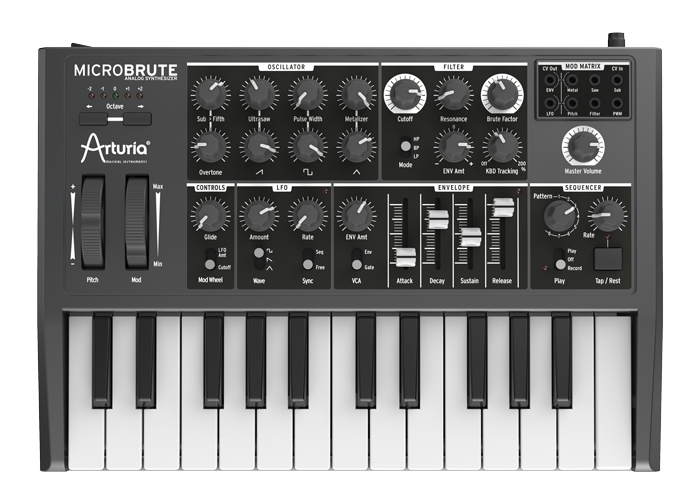
\includegraphics[width=2.5in]{analogSynth}
		\caption{Arturia Microbrute analog synthesizer with digital controls~\cite{analogSynth}. }
		\label{fig:analogSynth}
	\end{figure}
	
	Hybrid synths demonstrate the success of the digital-control-over-analog-audio-circuitry approach. They are readily integrated into computer-based recording studios. The G9 processor takes this hybrid approach to sound generation and applies it to sound processing.
	
	
	
	\section{Project Scope}
	
	Because most recording engineers use equalization (EQ), amplitude dynamic range compression (compressor), and ambience (reverb), the G9 will have each of those modules.
	
	\subsection{EQ}
	The EQ in the G9 will have high and low shelving filters based on a Baxandall circuit; Figure \ref{fig:baxandall} shows the circuit and its frequency response. It will also have a parametric midrange boost/cut with adjustable frequency. 
	
	
	\begin{figure}
		\centering
		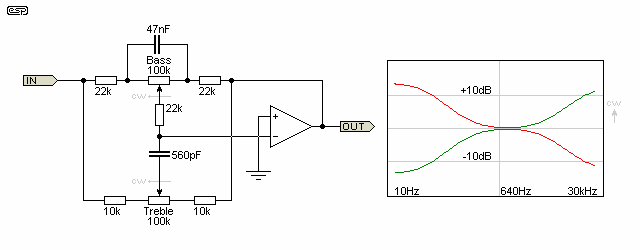
\includegraphics[width=2.5in]{baxandall}
		\caption{Baxandall filter circuit and frequency response~\cite{baxandall}. }
		\label{fig:baxandall}
	\end{figure}
	
	\subsection{Compressor}
	The compressor will be based on Teletronix LA-2A vacuum tube leveling amplifier. This circuit has two main elements that give it its characteristic sound. First, a gain element is controlled by a combination of an electroluminescent panel and a photo-resistor. The non-linear response curve of that combination results in a very pleasing sound of the gain reduction.  Second, tubes distort the signal in a musical way when the signal level pushes them out of their linear operating zone. Figure \ref{fig:OpticalAttenuator} shows the operating principle of the compressor.
	
	Drip Electronics has developed an updated version of the LA-2A compressor and sells a PCB of their design as well as a PCB for the power supply of the compressor. We already have these PCBs (figures \ref{fig:opto7pcb} and \ref{fig:opto7powerpcb}) and now need to acquire the parts and assemble the unit.
	
	\begin{figure}
		\centering
		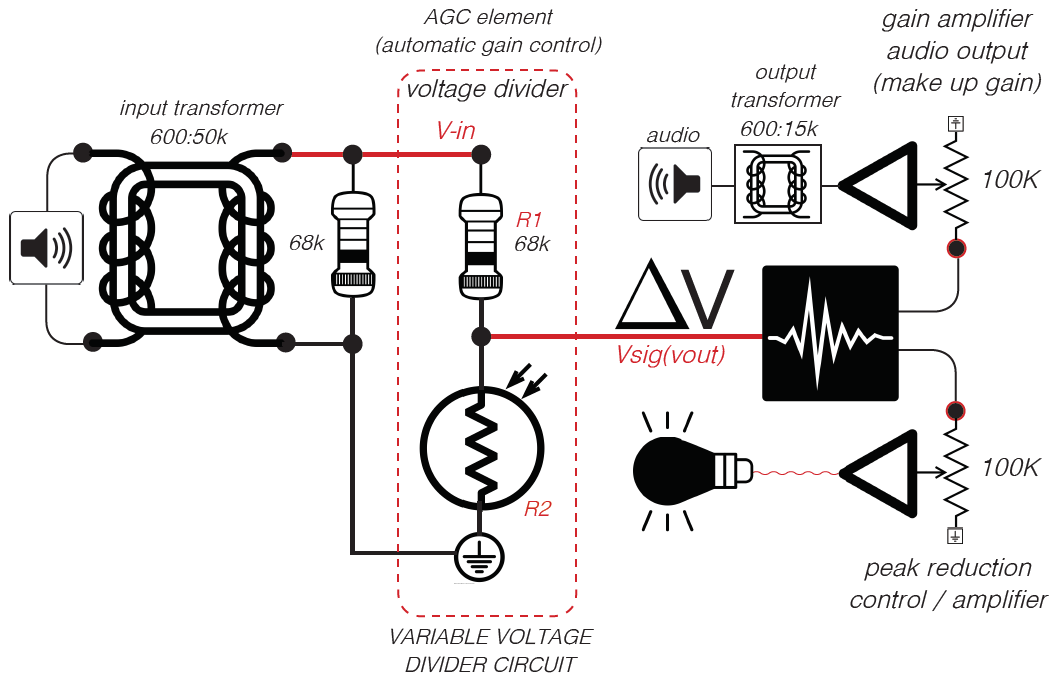
\includegraphics[width=3in]{OpticalAttenuator}
		\caption{Operating principle of the compressor's optical attenuator~\cite{opto7}. }
		\label{fig:OpticalAttenuator}
	\end{figure}
	
	
	\begin{figure}
		\centering
		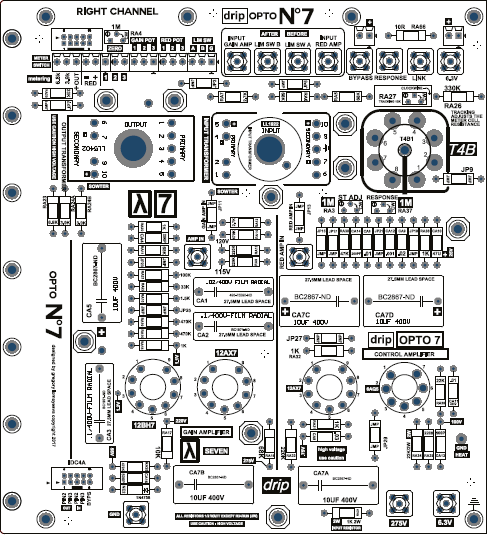
\includegraphics[width=3in]{opto7pcb}
		\caption{PCB of the compressor circuit~\cite{opto7}. }
		\label{fig:opto7pcb}
	\end{figure}

	\begin{figure}
		\centering
		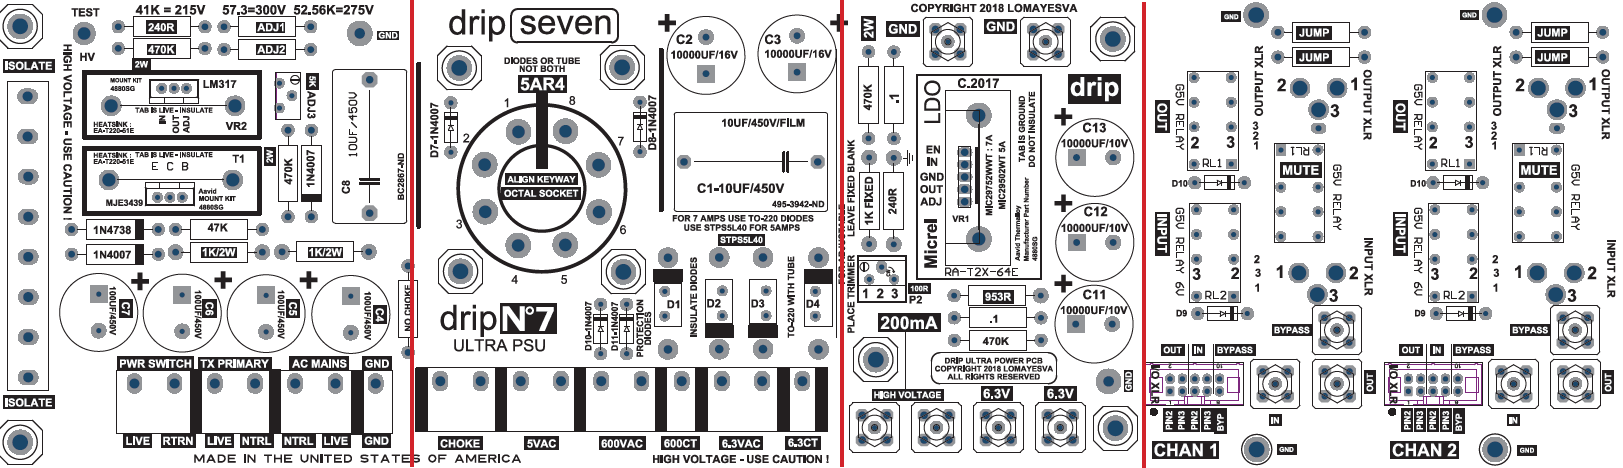
\includegraphics[width=3.4in]{opto7powerpcb}
		\caption{PCB of the compressor's power supply~\cite{opto7}. }
		\label{fig:opto7powerpcb}
	\end{figure}
	

	
	\subsection{Reverb}
	Reverb options are limited in the analog domain. The favored option is to place a loudspeaker in one part of a reverberant chamber and place a microphone in another part. When sound is played through the loudspeaker it is reverberated by the chamber and picked up by the microphone. Reverb of this sort is not feasibly placed inside an enclosure for use in a studio. 
	
	The sound of reverb is generally divided into two parts: early reflections and late reflections~\cite{earlyReflections}. Early reflections are heard as discrete echos, as when sound bounces off the walls of a chamber. Late reflections are heard after the early reflections as the early reflections build up and fuse into a wash of sound. This part of the reverb is also known as the tail. The time it takes for the tail to fade by 60 dB below the initial sound level is specified as the reverb time. The G9 will combine two methods to achieve a simulation of the chamber's early reflections and reverb tail.
	
	\begin{figure}
		\centering
		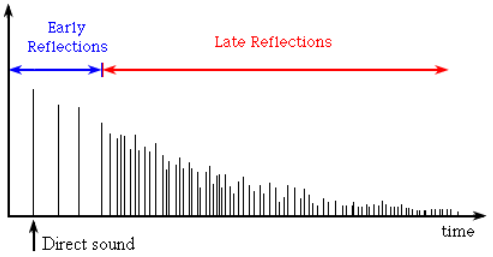
\includegraphics[width=3in]{earlyReflections}
		\caption{Impulse response of a typical reverb signal~\cite{vocalEarlyReflections}. }
		\label{fig:earlyReflections}
	\end{figure}
	
	A hose delay will be used for the early reflections. An amplifier will drive the audio signal through a balanced armature driver, like those used by in-ear monitors. The driver will be coupled to one end of a thin hose or tube. A microphone will be coupled to the other end. Sound played at one end will travel through the hose and be picked up by an electret microphone at the other end. Feedback can be used for sound reflections at a multiple of the delay time; multiple hose rigs can be used for specific reflections.
	
	An amplifier will take the signal from the microphone and drive it through a pair of springs to generate the dense, diffuse reflections that happen in a reverberant chamber after the sharp early reflections decay into a wash of sound. Figure \ref{fig:reverbBlock} shows a diagram of the reverb section of the G9. Amplifier schematics for the reverb are shown in figure \ref{fig:espMicPreSpringDrive}.
	
	\begin{figure}
		\centering
		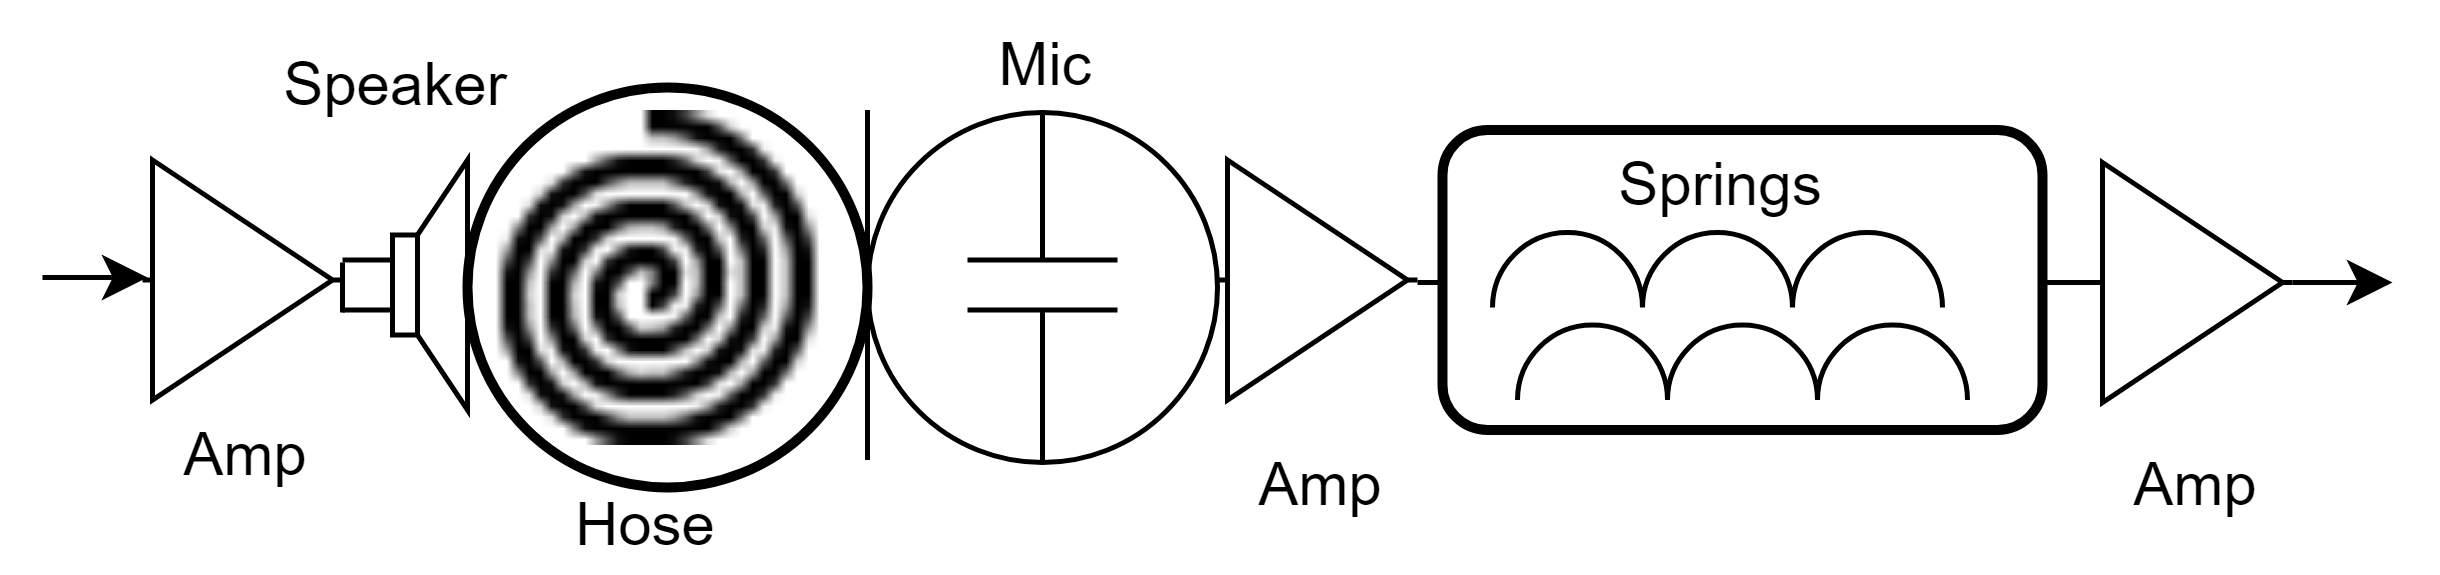
\includegraphics[width=3in]{reverbBlock}
		\caption{Diagram of the reverb section }
		\label{fig:reverbBlock}
	\end{figure}
	
	
	
	\begin{figure}
		\centering
		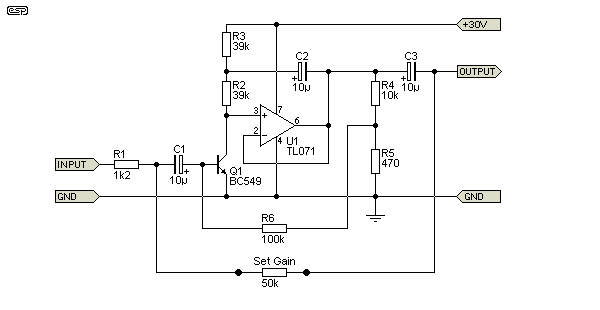
\includegraphics[width=3in]{espMicPreSpringDrive}
		\caption{Reverb amplifiers~\cite{espMicPreSpringDrive}. }
		\label{fig:espMicPreSpringDrive}
	\end{figure}
	
	\subsection{Digital Control}
	A graphical user interface (GUI) will run on a separate computer to send control signals to the G9's processing blocks. The computer will maintain the state of the system and be able to store and recall the state at any time. Figure \ref{fig:gui} shows a mockup of the G9's GUI.
	
	\begin{figure}
		\centering
		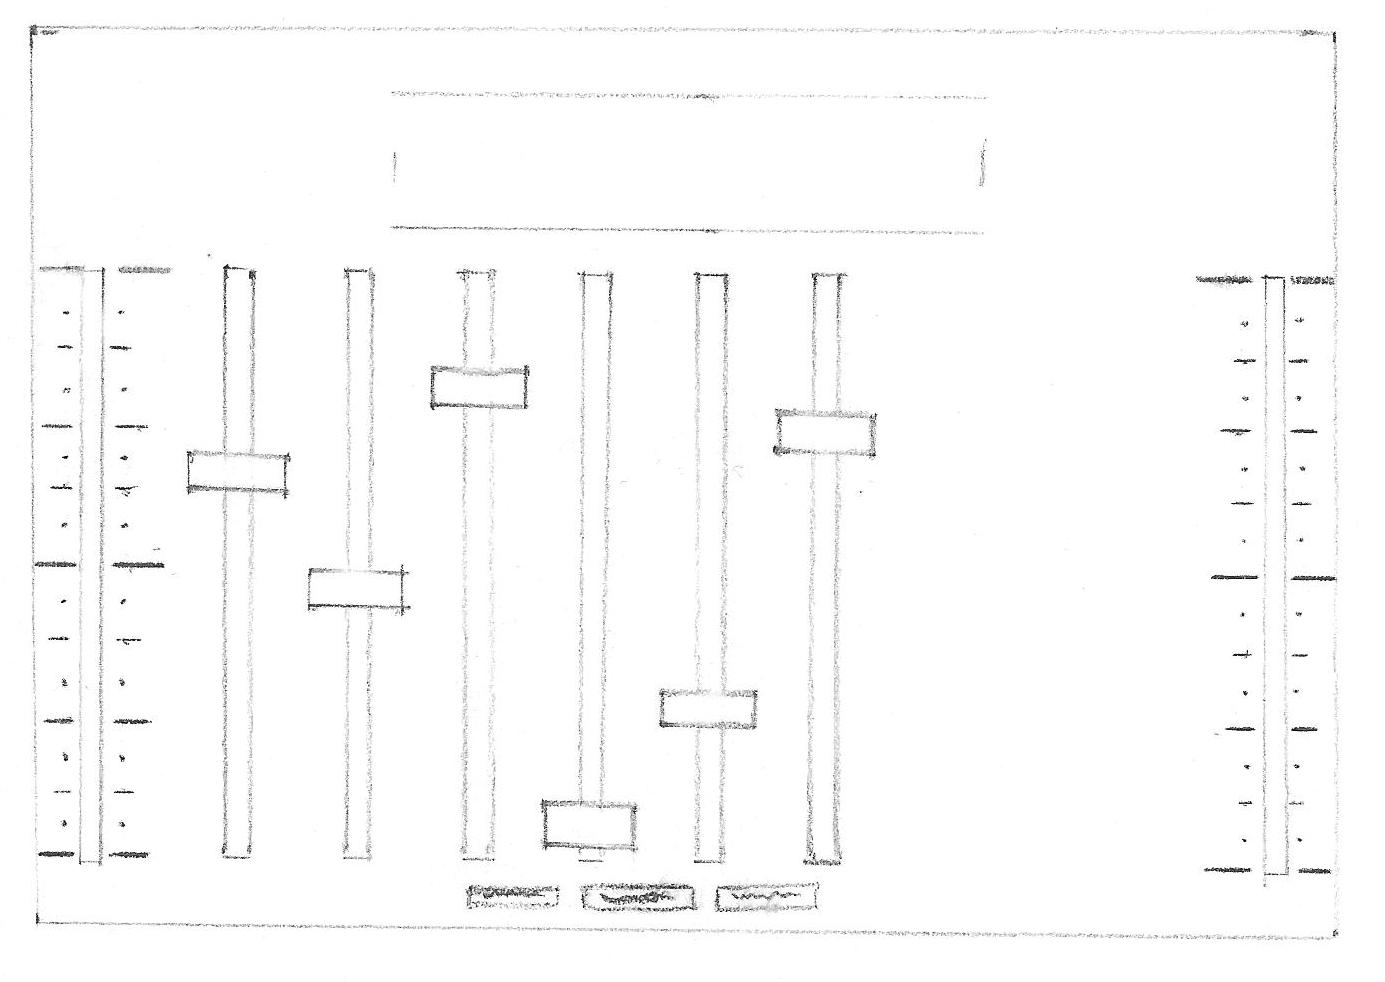
\includegraphics[width=2.5in]{gui}
		\caption{Mockup of the G9's GUI. }
		\label{fig:gui}
	\end{figure}
	
	
	\section{Design Approach}
	The G9 will utilize digital potentiometer ICs to control the parameters of its signal processors.  These ICs will be communicated to through I\textsuperscript{2}C or another serial protocol. An FPGA will provide processing for a graphical display separate from the GUI. The graphical display will show information about the sound level and frequency spectrum of the output audio signal itself. The GUI will have slider controls and show the state of the G9. A Raspberry Pi and will act as the CPU and take control signals from the GUI and route them to the appropriate digital potentiometers. Figure \ref{fig:blockDiagram} shows a block diagram of the G9.
	
	\begin{figure}
		\centering
		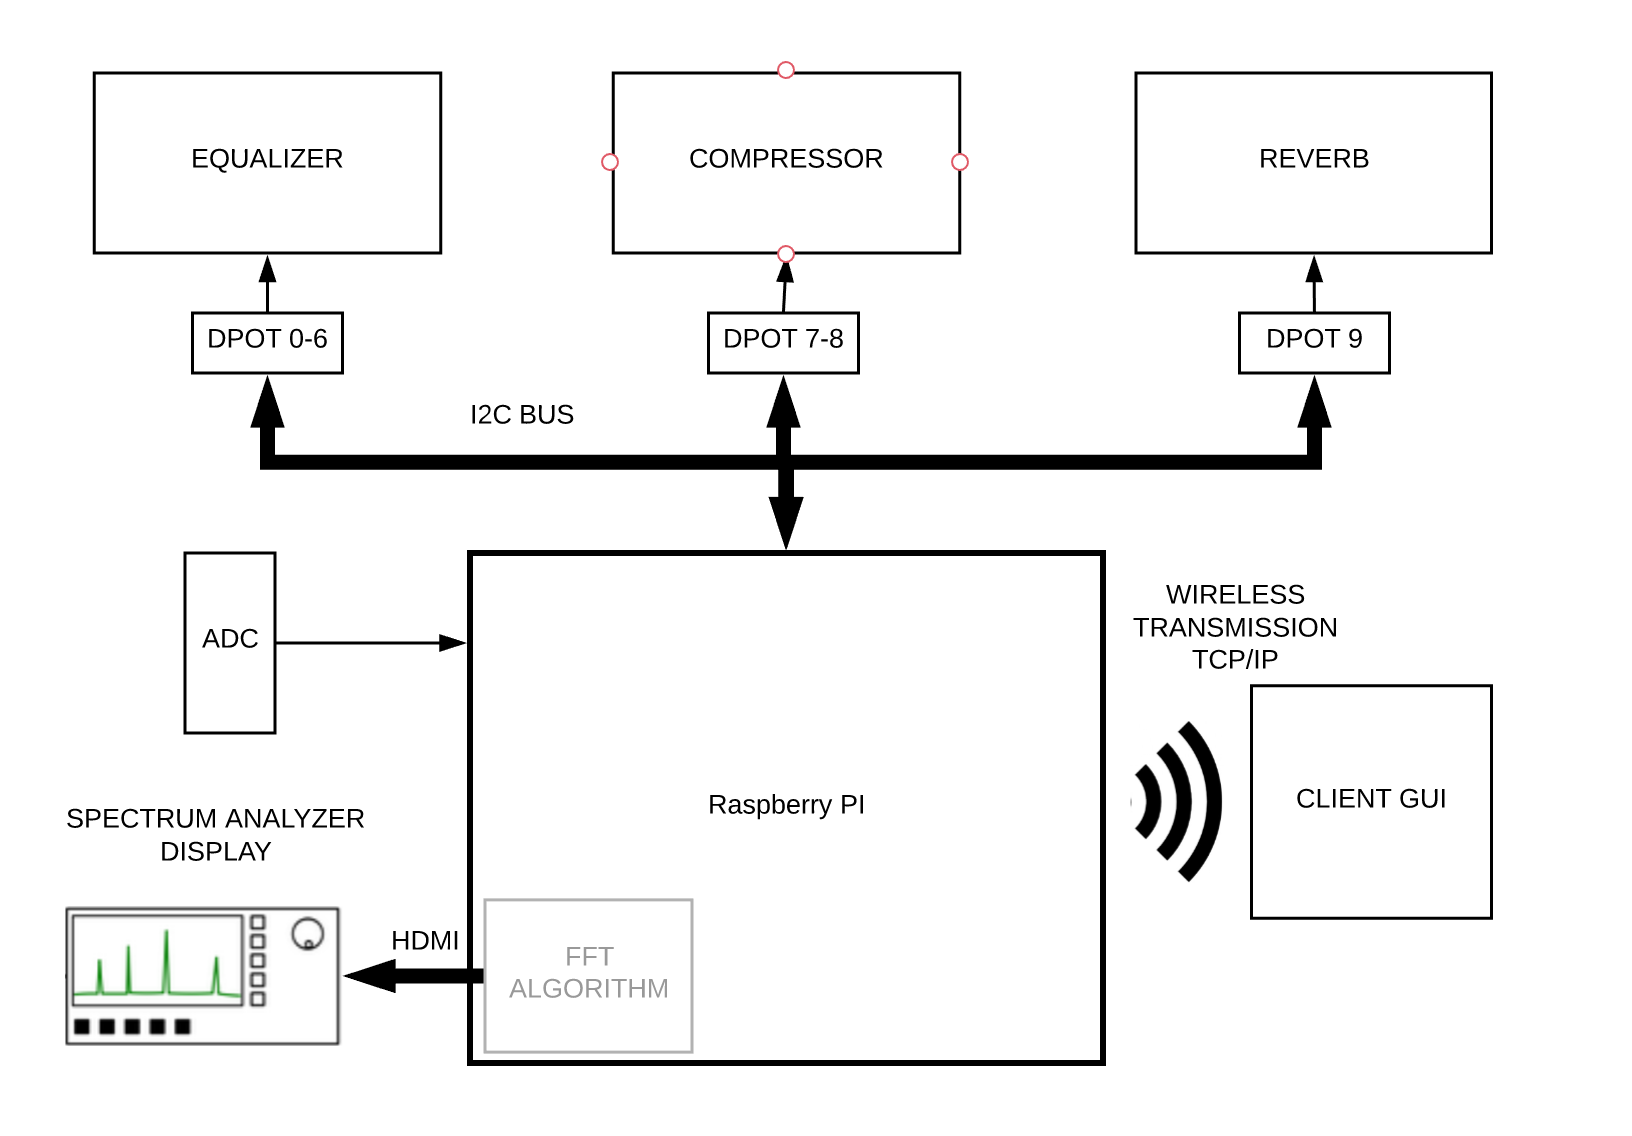
\includegraphics[width=2.5in]{blockDiagram}
		\caption{Block diagram of the G9. }
		\label{fig:blockDiagram}
	\end{figure}
	
	Figure \ref{fig:g9Enclosure} shows a mockup of the G9's enclosure. It will have LED meters showing input and output signal levels, an LED meter showing the compressor's gain reduction, and an LED meter showing the reverb's wet/dry signal balance. It will also have two rotary encoders to adjust the signal level going into the processor and the signal level coming out of the processor. The rotary encoders will allow for the changes to be saved with the GUI as well as for the state to be loaded easily.
	\begin{figure}
		\centering
		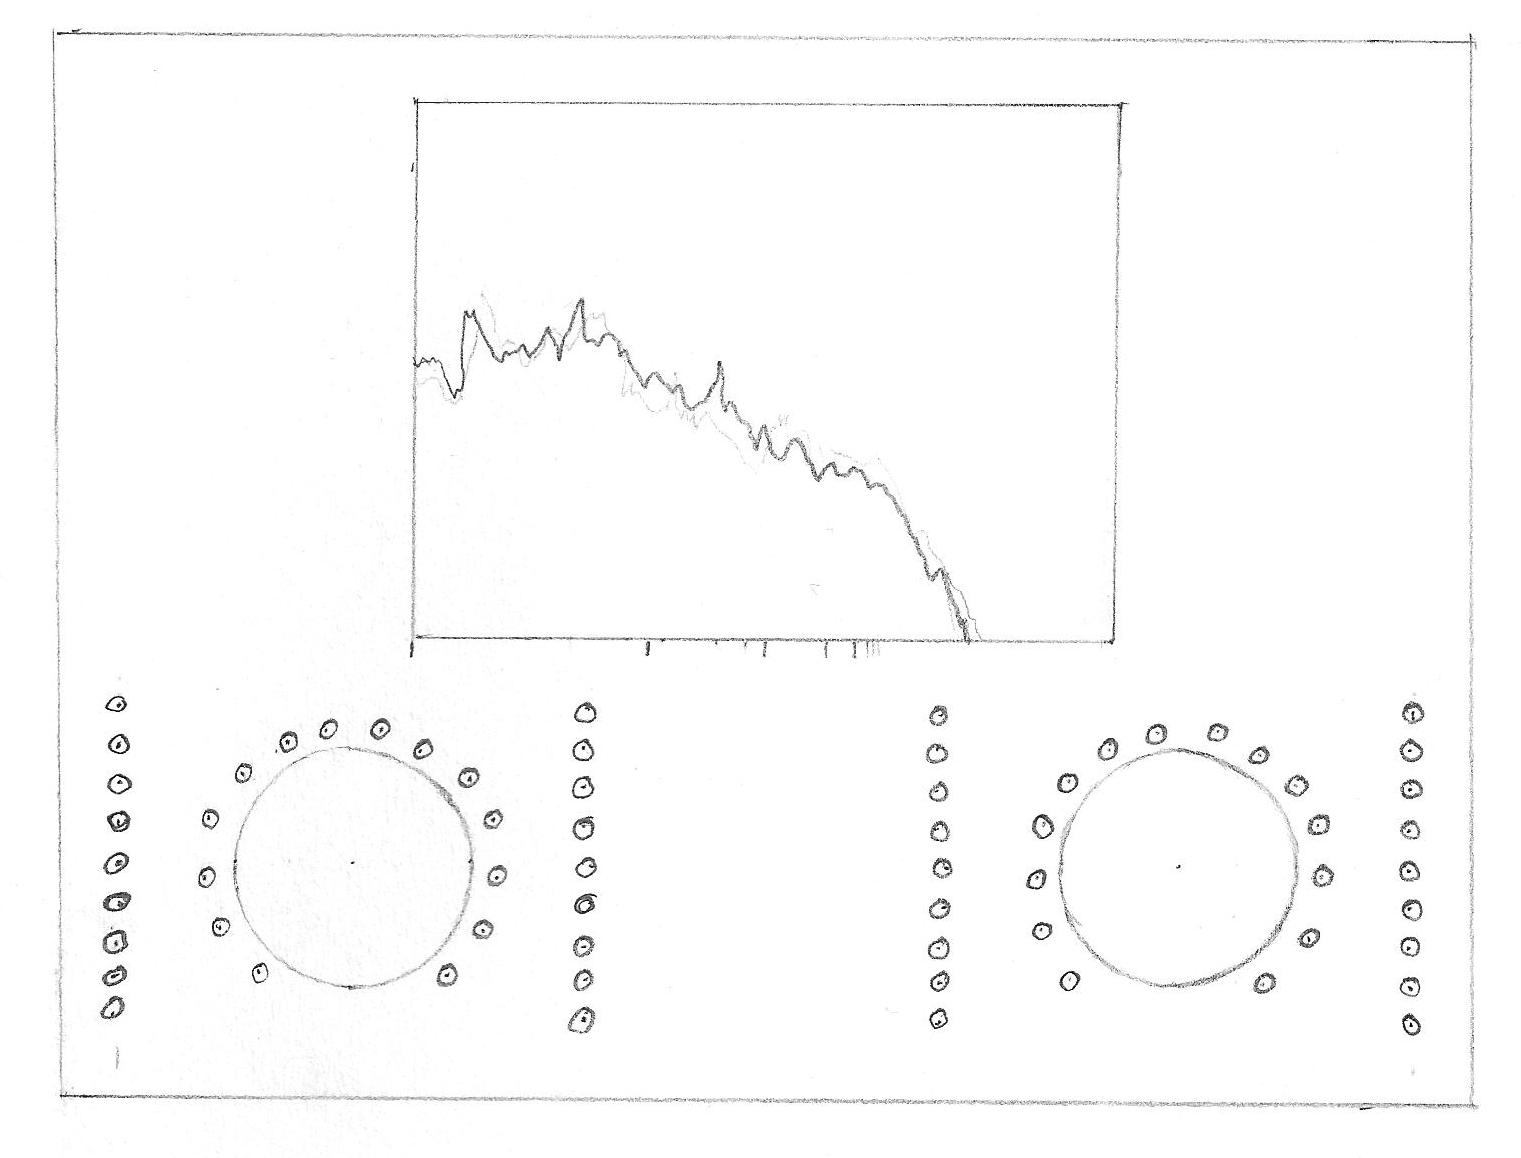
\includegraphics[width=2.5in]{g9Enclosure}
		\caption{Mockup of the G9's enclosure. }
		\label{fig:g9Enclosure}
	\end{figure}
	
	\section{Tasks}
	This is a list of the parts the project that will need to be completed.
	
	\begin{itemize}  
		\item EQ circuit 
		\item Compressor circuit
		\item Reverb circuit
		\begin{enumerate}
			\item Speaker into tube
			\item Microphone out of tube, piezo driver into spring
			\item Pickup out of spring to be mixed into main signal
		\end{enumerate}
		\item Digital control of the processors
		\item GUI
		\item Control parameters from GUI to CPU
		\item Control parameters from CPU to control signal generator
		\item LED meters on the G9 enclosure
		\item Rotary encoders and LEDs on the G9 enclosure
		\item FPGA analysis of the audio signal for display
		\item FPGA display driver
	\end{itemize}
	
	
	\section{Testing Plan}
	The G9 is highly modular. Each piece can be tested on its own to ensure it functions correctly before attempting to combine all the elements together. GUI, CPU, FPGA, display, EQ, compressor, reverb will all be tested on their own. When each component is functioning correctly on its own, then the pieces will be connected together one-by-one and tested.
	
	\section{Demo}
	A base demo of the G9 will consist of a sound playback device being plugged into the G9, and the output of the G9 will be plugged into a sound system. Each of the three sound processors will be demonstrated in turn by adjusting their parameters one by one on the GUI and listening to how the sound changes on the playback system. A more detailed demo will consist of a more in-depth presentation of how the GUI, control system, analog processors, and information display all work together.
	
	
	\section{Conclusion}
	Digital audio signal processors have processing latencies on the order of milliseconds. When multiple processors are used in recording studios, their interacting latencies can cause comb filtering or lengthy delays in the signals being processed. Analog audio processors have latencies on the order of nanoseconds and also are often preferred for the character of the sounds they produce. The problem with analog processors is that their controls are often manually operated potentiometers and switches. Some companies in the past have created products that take a hybrid analog/digital approach, but currently no product is available that maintains a fully analog audio signal path incorporating the main processing blocks desired by sound engineers. The G9 processor has the three main processing blocks of EQ, compressor, and reverb, and takes advantage of the low latency and sound quality of analog processing with the convenience and repeatability of digital control.
	
	
	
	
	
	
	% Can use something like this to put references on a page
	% by themselves when using endfloat and the captionsoff option.
	\ifCLASSOPTIONcaptionsoff
	\newpage
	\fi
	
	
	
	\bibliographystyle{ieeetran}
	\bibliography{g9}
\end{document}
